\documentclass{beamer}
\usetheme{metropolis}

% Layout/Format
\usepackage{multirow}
% Math/Algorithms
\usepackage{amsmath}
\usepackage{amsthm}
\usepackage{amssymb}
\usepackage{algorithm2e}
% Graphics
\usepackage{float}
\usepackage{graphicx}
\usepackage{tikz}
% Utility
\usepackage{dirtytalk}
\usepackage{xcolor}
% Language & Symbols
\usepackage[utf8]{inputenc}
\usepackage[T1]{fontenc}
\usepackage[english]{babel}
\usepackage{wasysym}
\usepackage[absolute,overlay]{textpos}

\title{Graph Drawing}
\date{\today}
\author{Calvin Bulla \\ Enrique Díaz Roque}
\institute{Algorithms for VSLI}

\begin{filecontents}{refs.bib}
@inproceedings{walshaw2000multilevel,
  title={A multilevel algorithm for force-directed graph drawing},
  author={Walshaw, Chris},
  booktitle={International Symposium on Graph Drawing},
  pages={171--182},
  year={2000},
  organization={Springer}
}
@article{gallier2014elementary,
  title={Elementary Spectral Graph Theory Applications to Graph Clustering Using Normalized Cuts: a Survey},
  author={Gallier, Jean and Gallier, C Jean},
  year={2014},
  publisher={Citeseer}
}

\end{filecontents}

\newcommand*{\describe}[1]{$\diamond$ \textbf{#1}\ }

\begin{document}
\maketitle

\begin{frame}
\begin {enumerate}
\item Where (class topic) ~ Global and detailed placement ~ Force directed placement (class theory)
\item Our setup
\item Graph drawing
\item Initial position
\item Iterative process
\item Forces
\item Repulsive
\item Spring
\item Parallelism
\item Experiments modifying functions (forces)
\item Experiments scaling topology
\item Experiments convergence
\item Extensions (clustering, optimizations, details that we didn’t have time to implement (but we liked), …)
\item Conclusion
\end{enumerate}
\end{frame}

\begin{frame}{Introduction}
\begin{itemize}
\item Global and detailed placement
\item Analytic tecnique
\begin{itemize}
\item Quadratic placement
\item Force-directed placement
\end{itemize}
\end{itemize}

\centering
\includegraphics[width=0.6\textwidth]{images/placement.png}

\end{frame}

\begin{frame}{Initial positioning}
\centering
\only<1>{
Start with a symmetric topology matrix\\\vspace{2em}
$
A=
 \begin{pmatrix}
  0 & 1 & 1 & 0 \\
  1 & 0 & 0 & 1 \\
  1 & 0 & 0 & 1 \\
  0 & 1 & 1 & 0 \\
 \end{pmatrix}
$
}
\only<2>{
Weight of A in diagonal\\\vspace{2em}
$
D=
 \begin{pmatrix}
  2 & 0 & 0 & 0 \\
  0 & 2 & 0 & 0 \\
  0 & 0 & 2 & 0 \\
  0 & 0 & 0 & 2 \\
 \end{pmatrix}
$
}
\only<3>{
Unnormalized Laplacian matrix associated with A\\\vspace{2em}
$
L=D-A=
 \begin{pmatrix}
  2 & -1 & -1 & 0 \\
  -1 & 2 & 0 & -1 \\
  -1 & 0 & 2 & -1 \\
  0 & -1 & -1 & 2 \\
 \end{pmatrix}
$
}
\only<4>{
We obtain eigenvalues of L such that\\\vspace{2em}
$
0=\lambda_1 \leq \lambda_2 \leq \lambda_3 \leq ... \leq \lambda_m
$
}
\only<5>{
It is known that the minimal energy of any blanced orthogonal graph in ${\rm I\!R}^n$ is\\\vspace{2em}
$
0= \lambda_2 + ... + \lambda_{n+1}
$\\\vspace{2em}
hence, the eigenvectors associated yields a blanced orthogonal graph drawing of minimal energy
}

\only<6>{
Eigenvalues and eigenvectors of L\\\vspace{2em}
$
E=
 \begin{pmatrix}
  4 & 0 & 0 & 0 \\
  0 & 2 & 0 & 0 \\
  0 & 0 & 2 & 0 \\
  0 & 0 & 0 & 0 \\
 \end{pmatrix}
$
\\\vspace{1em}
$
V=
 \begin{pmatrix}
   0.50000 &  0.67458 & -0.21200 & 0.50000 \\
  -0.50000 &  0.21200 &  0.67458 & 0.50000 \\
  -0.50000 & -0.21200 & -0.67458 & 0.50000 \\
   0.50000 & -0.67458 &  0.21200 & 0.50000 \\
 \end{pmatrix}
 $
}

\only<7>{
\centering
\includegraphics[width=0.8\textwidth]{images/rectangle.png}
}

\end{frame}

\begin{frame}{Extensions/Optimizations}
Embarassingly parallel algorithm:
\begin{itemize}
  \item Double buffering (no read/write conflicts)
  \item Independent computation for each node
\end{itemize}
$\Rightarrow$ Split work between multiple cores (shared memory)

\begin{center}
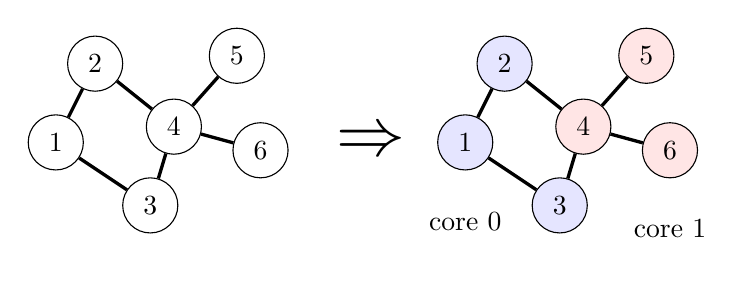
\begin{tikzpicture}[
  every node/.style={draw,circle,minimum width=7mm},
  edge/.style={very thick}
  ]

  \begin{scope}
    \node (a) at (0,0)      {1};
    \node (b) at (0.5,1)    {2};
    \node (c) at (1.2,-0.8) {3};
    \node (d) at (1.5,0.2)  {4};
    \node (e) at (2.3,1.1)  {5};
    \node (f) at (2.6,-0.1) {6};

    \draw[edge] (a) -- (b);
    \draw[edge] (b) -- (d);
    \draw[edge] (a) -- (c);
    \draw[edge] (c) -- (d);
    \draw[edge] (d) -- (e);
    \draw[edge] (d) -- (f);

    \node[draw=none] at (4,0) {\Huge$\Rightarrow$};
  \end{scope}
  \begin{scope}[xshift=5.2cm]
    \node[fill=blue!10] (a) at (0,0)      {1};
    \node[fill=blue!10] (b) at (0.5,1)    {2};
    \node[fill=blue!10] (c) at (1.2,-0.8) {3};
    \node[fill=red!10] (d) at (1.5,0.2)  {4};
    \node[fill=red!10] (e) at (2.3,1.1)  {5};
    \node[fill=red!10] (f) at (2.6,-0.1) {6};

    \node[draw=none, below of=a] {core 0};
    \node[draw=none, below of=f] {core 1};

    \draw[edge] (a) -- (b);
    \draw[edge] (b) -- (d);
    \draw[edge] (a) -- (c);
    \draw[edge] (c) -- (d);
    \draw[edge] (d) -- (e);
    \draw[edge] (d) -- (f);
  \end{scope}
\end{tikzpicture}
\end{center}
\end{frame}

\begin{frame}{Extensions/Optimizations}
  Clustering\dots
  \centering
  \includegraphics[width=0.6\textwidth]{images/clustering.png}
\end{frame}

\nocite{*}

\begin{frame}{References}
  \bibliographystyle{amsalpha}
  \bibliography{refs.bib}
\end{frame}

\end{document}
